\documentclass[11pt]{article}

\usepackage{thumbpdf, amssymb, amsmath, amsthm, microtype,
	    graphicx, verbatim, listings, color, fancybox}
\usepackage[pdftex]{hyperref}
%\usepackage[margin=1in]{geometry}
\usepackage{cawsty}
\usepackage{fullpage}
\usepackage{pseudocode}
\usepackage{fancybox, fancyvrb}

\newcommand{\field}[1]{\mathbb{#1}} %requires amsfonts

%\setlength{\parindent}{0pt}

\linespread{1.2}

\begin{document}
\cawtitlelong{4040-849 Optimization Methods}{Optimizing Cryptographic Strength of Substitution}{Layers in Symmetric-Key Cryptosystems}

\begin{abstract}
The cryptographic security of symmetric-key block ciphers and other related primitives is based upon their adherence to Shannon's principles of confusion and diffusion \cite{Kim90astudy}. Confusion can be defined as the statistical relationship between the ciphertext and private key of a cipher, while diffusion refers to the statistical redundancy of plaintext bits in the ciphertext bits. Consequently, it is increasingly important to optimize these characteristics in order to make them less susceptible to attacks based on linear and differential cryptanalysis. S(ubstitution)-boxes are the most traditional mathematical structures that are used to improve the levels of diffusion and confusion within symmetric-key cryptographic algorithms. Recent research efforts have revealed practical measurements of S-box constructions that indicate their susceptibility to linear and differential cryptanalysis. In this work, we attempt to formulate the problem of cryptographically strong substitution layers in symmetric-key block ciphers with S-box designs into a mixed integer programming problem that can be optimized to yield the high diffusion and confusion dividends in resulting cipher implementations.
\end{abstract}

\section{Problem Description}
The strength of cryptographic algorithms is commonly measured by their resilience to common cryptanalysis attacks, such as linear and differential cryptanalysis. Linear cryptanalysis is is an attack that attempts to take advantage of high probability occurrences of linear expressions involving plaintext bits, ciphertext bits, and subkey bits. Mathematically, the attack is based on the idea of approximating the operation of a portion of the block cipher in question with an expression that is linear in terms of the input ($X$) and output ($Y$) bits involved, as shown below \cite{Heys01atutorial}:
\begin{eqnarray*}
X_{i_{1}} \oplus X_{i_{2}} ... \oplus X_{i_{r}} \oplus Y_{j_{1}} \oplus Y_{j_{2}} ... \oplus Y_{j_{s}} \oplus  = 0
\end{eqnarray*}
Using this expression, attackers can guage the amount of randomness introduced by the cipher. That is, if such an expression is satisfied frequently (with a relatively high probability), then we know that the probability of the expression holding for any two values $a,b\in \field{F}_2^n$ is approximately $\frac{1}{2}$. However, when this probability shifts away from $\frac{1}{2}$, the amount of known plaintexts required to determine the key (or key block) that was used to reproduce the output goes down dramatically. Such a deviation from the expected probability of $\frac{1}{2}$ for any expression of the form above, which is referred to as the \emph{linear bias}, determines the susceptibility of the block cipher to known plaintext attacks. Therefore, it is important to introduce non-linearity into the block cipher in order to defend against such attacks.

Differential cryptanalysis is a very powerful attack technique that attempts to break symmetric key ciphers by exploiting high probability of certain occurrences of plaintext differences and ciphertext differences \cite{Heys01atutorial}. To illustrate this attack technique, consider the input of a block cipher to be represented by the vector $[X_1, X_2,..., X_n]$ and the corresponding output to be $[Y_1, Y_2, ..., Y_n]$, where each element $X_i$ and $Y_i$ corresponds to a single bit in the input and output, respectively. With this definition, we can represent the input difference of any two input vectors ($\Delta X$) and any two output vectors ($\Delta Y$) as follows:
\begin{eqnarray*}
\Delta X = [\Delta X_1 \oplus \Delta X_2 \oplus ... \oplus \Delta X_n]  \\
\Delta Y= [\Delta Y_1 \oplus \Delta Y_2 \oplus ... \oplus \Delta Y_n]
\end{eqnarray*}
where $\Delta X_i = X_{i,1} \oplus X_{i,2}$ and $\Delta Y_i = Y_{i,1} \oplus Y_{i,2}$. It is an ideal block cipher the output different $\Delta Y$ for a specific input different $\Delta X$ will occur with a probability of approximately $\frac{1}{2^n}$ (i.e. it produces random output based on every input block). Note that it is common to represent the input and output difference pairs as $(\Delta X, \Delta Y)$ (which are referred to as differentials).

With the idea of differential pairs in mind, we define differential cryptanalysis as the process of finding differentials that occur with a probability much higher than $\frac{1}{2^n}$, which subsequently gives rise to a statistical correlation between the relationship between the input and output of a block cipher and can allow one to deduce the private key used in the cipher. Therefore, it is ideal to maximize the amount of randomness introduced by the block cipher through each iteration. Clearly, this necessity can be traced back to the need for high diffusion and confusion levels in block ciphers.

The efficiency of both of these attacks relate to the measures of confusion and diffusion within a cipher and the extent to which they can be exploited. Confusion is typically referred to as the complexity of the relationship between the secret-key and ciphertext, and diffusion is commonly referred to as the degree to which the influence of a single input bit is spread throughout the resulting ciphertext. In the context of cryptographic algorithms, these characteristics are usually realized through a unique combination of linear and nonlinear operations. It is clear that the nonlinear operations in the algorithms contribute more to the security of the corresponding algorithm than the other components. The most common source of nonlinearity in symmetric-key cryptographic algorithms is from a S(ubstitution)-box, which is a function with an equal sized domain and range that is configured to yield optimal confusion and diffusion between each input and output pair. As such, S-boxes (as the substitution layer in cryptographic algorithms) will be the focus of this project. 

\subsection{Cryptographic Strength of Substitution Layers}
Mathematically, an S-box can be represented as a function $f$ that maps input values $a$ to output values $b$ such that $a,b \in \field{F}_2^n$. In the context of cryptographic applications, such a function $f$ should be bijective in order to avoid bias towards any specific output element in the field. We now present a series of definitions that are pertinent to the design of cryptographically strong S-Boxes \cite{Mar_newanalysis}.

%TODO: http://www.waset.org/journals/waset/v48/v48-24.pdf && thesis work

\begin{define}
The \emph{Hamming weight} of an element $x \in \field{F}_2^n$ is defined as wt$(x) = \sum x_i$, where $x_i$ refers to the $i$th bit in $x$.
\end{define}

\begin{define}
Let $f$ be a bijective function with range $\mathbb{R^*}$, where $|\mathbb{R^*}| = m$. Let $n$ be the number of elements $x$ that satisfy $f(x \oplus \Delta_i) = f(x) \oplus \Delta_o$. Then, $\frac{n}{m}$ is the \emph{differential probability p} of the characteristic $f_D(\Delta_i \to \Delta_o)$.
\end{define}

\begin{define}
The \emph{branch number} of an $n \times n$-bit S-Box is
\begin{eqnarray*}
BN = \text{min}_{a, b\not=a}(\text{wt}(a \oplus b) + \text{wt}(S(a) \oplus S(b))),
\end{eqnarray*}
where $a, b \in \field{F}_2^n$.
\end{define}

\begin{define}
A function $f : \field{F}_2^n \to \field{F}_2^n$ exhibits the \emph{avalanche effect} if and only if 
\begin{eqnarray*}
\sum_{x \in \field{F}_2^n} \text{wt}(f(x) \oplus f(x \oplus c_{i}^{n})) = n2^{n-1},
\end{eqnarray*}
for all $i (1 \leq i \leq n)$, where $c_{i}^{n} = [0, 0, ..., 1, ..., 0]$ (where a $1$ is in the $n$th position of the vector of cardinality $n$).
\end{define}

\begin{define}
A function $f : \field{F}_2^n \to \field{F}_2^n$ satisfies the \emph{Strict Avalanche Critertion (SAC)} if for all $i (1 \leq i \leq n)$ the following equations hold:
\begin{eqnarray*}
\sum_{x \in \field{F}_2^n} f(x) \oplus f(x \oplus c_i^n) = (2^{n-1}, 2^{n-1}, ..., 2^{n-1})
\end{eqnarray*}
This simply means that $f(x) \oplus f(x \oplus c_i^n)$ is balanced for every element in $\field{F}_2^n$ with Hamming distance of $1$. 
\end{define}

\begin{define}
The \emph{degree of nonlinearity} of an $n \times n$-bit S-Box from $\field{F}_2^n \to \field{F}_2^n$ can be measured by
\begin{eqnarray*}
	P_S = \text{max}_{0 \not= a, b}|\{x \in \field{F}_2^n : S(x + a) - S(x) = b\}|
\end{eqnarray*}
where $a, b \in \field{F}_2^n$, and a low measure for $P_S$ indicates a high degree of nonlinearity.
\end{define}

Designers of cryptographically secure cryptographic primitives (e.g. block ciphers, hash functions, etc) use all of these measurements as a basis for the degrees of confusion and diffusion within a cipher, and thus for their susceptibility to linear and differential cryptanalysis (among other attacks). Specifically, it has been shown that cryptographically secure symmetric-key algorithms utilize substitution layers that provide the following characteristics:
\begin{enumerate}
	\item Low differential propagation probability
	\item High branch number
	\item High satisfaction of the SAC criterion
	\item High degree of nonlinearity
\end{enumerate}
However, in practice the additional constraints that fast and simple mathematical operations must be used to emulate represent such a bijective function $f$ that exhibits ideal values for all of these measurements.

\section{Optimization Candidate and Problem Formation}
%TODO: discuss time complexity of each operation, infeasibility for higher order S-boxes
%TODO: discuss why exhaustive search is best (cryptographic strength, might be just one global max for joint computations)
%TODO: include brute force results for order4 here (separate and joint)
%TODO: summarize genetic algorithm approach, state each optimization problem as a MINLP problem
%1. state need to exhaust entire solution, but that's infeasible.
%2. state optimization problems for each one separately
%3. state optimization problem together as joint
%4. state solution is to use genetic algorithm and BB
%5. discuss genetic algorithm crossover and mutation

Due to the application of S-boxes inside cryptographic algorithms, it is ideal that such function configurations exhibit the globally maximum values for each of these metrics. The best way to achieve this assurance is to perform an exhaustive search over the S-box design space (i.e. consider all possible input and output values and find the one that yields the optimum results). The results from an exhaustive search for a $2$-bit S-box are shown in Figure \ref{bfjoint}

\begin{center}
	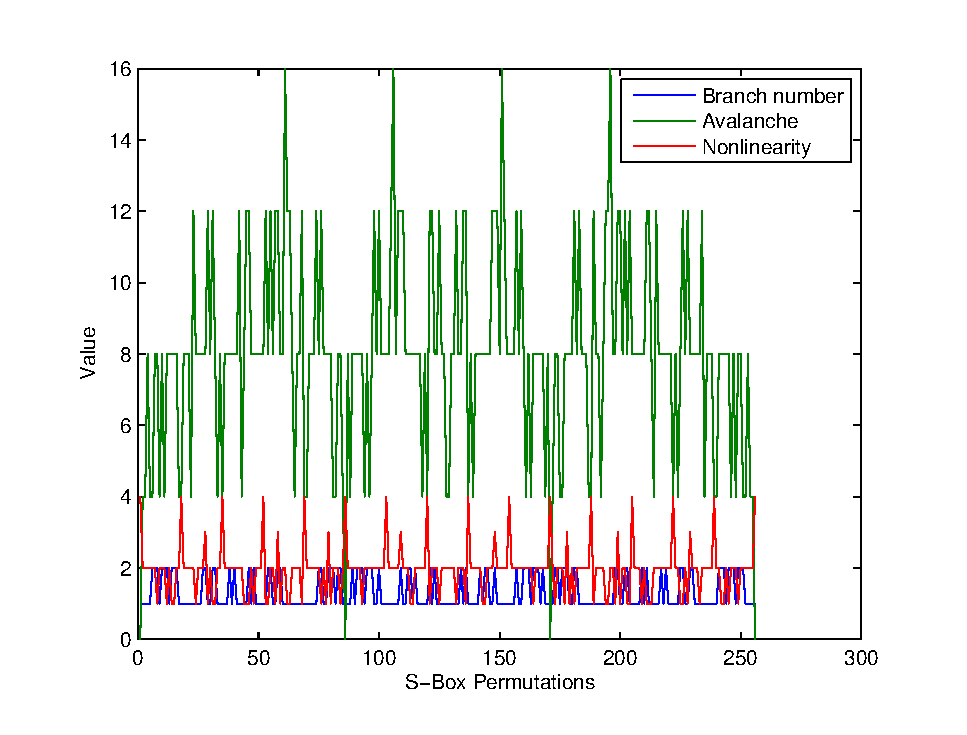
\includegraphics[scale=0.75]{images/brute_joint.eps} \\
	\label{bfjoint}
The results for the branch number, avalanche, and nonlinearity measurements for a $2$-bit S-box over all possible permutations in the design variables. 
\end{center}

Such exhaustive searches have a time complexity of $O(n^n)$ and thus are only feasible for small order S-boxes. However, recent research has advanced the upper bound on these exhaustive searches to include $4$-bit S-boxes, which were run in TODO: DETAILS (CITE cryptanalysis of 4x4 bit sboxes). Furthermore, due to the instability of each function over the design variable permutation space, it is clear that a probabilistic optimization algorithm would be best suited to optimizing each of these metrics. Before such an algorithm can be applied, however, we must formalize each objective function for these metrics as standard optimization problems. Treating each objective function as a mixed-integer nonlinear optimization problem yields the following problem definitions. \\

\shadowbox{%
\parbox{15cm}{% 
\textbf{Minimize}
\begin{eqnarray*}
BN'(X) = -BN(X) = -\text{min}_{i, j\not=i}(\text{wt}(i \oplus j) + \text{wt}(X(i) \oplus X(j))),
\end{eqnarray*}
subject to the constraints
\begin{eqnarray*}
0 \leq X(i) \leq 2^{n} - 1,
\end{eqnarray*}
where $n$ is the number of design variables.
}}

\shadowbox{%
\parbox{15cm}{% 
\textbf{Minimize}
\begin{eqnarray*}
A'(X) = -A(X) = -\sum_{x \in \field{F}_2^n} \text{wt}(f(x) \oplus f(x \oplus c_{i}^{n})),
\end{eqnarray*}
subject to the constraints
\begin{eqnarray*}
0 \leq X(i) \leq 2^{n} - 1,
\end{eqnarray*}
where $n$ is the number of design variables. \\
}}

\shadowbox{%
\parbox{15cm}{% 
\textbf{Minimize}
\begin{eqnarray*}
P_S(X) = \text{max}_{0 \not= a, b}|\{x \in \field{F}_2^n : S(x + a) - S(x) = b\}|
\end{eqnarray*}
subject to the constraints
\begin{eqnarray*}
0 \leq X(i) \leq 2^{n} - 1,
\end{eqnarray*}
where $n$ is the number of design variables. \\
}}

\section{Algorithm configuration}
%1. GA description - TODO: write up some characteristics of this algorithm
%2. BB description - TODO: write up some characteristics of this algorithm
\subsection{Genetic Algorithm}

Given the instability of each of these functions over the permutation design variable space, it is natural to solve these MINLP problem using a probabilistic optimization algorithm. For the purposes of this project, the main results were derived using a highly probabilistic genetic algorithm that attempts to explore the permutation design space as much as possible in search for the global optimum values. Genetic algorithms are commonly utilized in the context of cryptography to explore the design space for cryptographic functions. They serve as an intelligence optimization method that can ease the computational efforts of performing brute force searches among the design space, which is crucial for functions with larger domains. (CITE SHA-3 CANDIDATE UPDATE).

Since each of the aformentioned objective functions exhibit the same instable behavior, it is possible to apply the same genetic algorithm structure to solve each one of these. In particular, the genetic algorithm configuration for each of these problems used the following parameters.

\begin{table}
    \begin{tabular}{|l|l|}
        \hline
        \textbf{Algorithm option} & \textbf{Configuration} \\ \hline
        Population creation function & TODO: describe \\ 
        Population mutation function & TODO: describe \\ 
        Generations & $500$ \\ 
        Tolerance Function limit & $1 \times 10^{-6}$ from last function value change \\ 
        Stall generation limit & $2^{n^n}$ identical function values \\ 
        Initial population & S-box configuration $\langle 0, 1, ..., n \rangle$ \\
        \hline
    \end{tabular}
\end{table}

\subsection{Non-Probabilistic Optimization Algorithms}
%4. discuss why BB algorithm didn't work (converged too early and didn't exhaust, too many local minimums for every objective function, GA was good because it generated populations and did psuedo brute force thing)

The \emph{Branch and Bound} algorithm is another optimization algorithm commonly used to solve MINLP problems. However, this algorithm is not suitable in the context of this problem for a variety of reasons, as shown below.

\begin{enumerate}
	\item The branch and bound algorithm is greedy, in that it selects the appropriate decision branch to take to proceed towards the optimal value based on the current configuration. While this leads the algorithm towards an optimum value, it is usally a locally optimal solution. Furthermore, there is no penalty applied to the decision process that enables the design variables to change. 
	\item As shown in Figure \ref{bfjoint}, there are many locally optimum values for each objective function even with small order S-boxes. The usefulness of the BNB algorithm will surely degrade as larger order S-boxes are considered, because the number of intermediate local optimum values will increase significantly as well. This would cause the algorithm to converge to an optimal value too quickly and terminate with very few iterations. 
	\item TODO: what else
\end{enumerate}

OQNLP: stochastic process that relies on smoothness of function to approximate

\section{Optimization Results}
%TODO: compare GA results against exhaustive search and BB algorithm
%1. prsent individual and joint results for order 8 and 16  (3-bit and 4-bit S-boxes)
%2. discuss how close they got to optimal results
%3. discuss usefulness of GA
%4. discuss why BB algorithm didn't work (converged too early and didn't exhaust, too many local minimums for every objective function, GA was good because it generated populations and did psuedo brute force thing)

\subsection{Avalanche Number}
TODO: insert code/charts

\begin{center}
	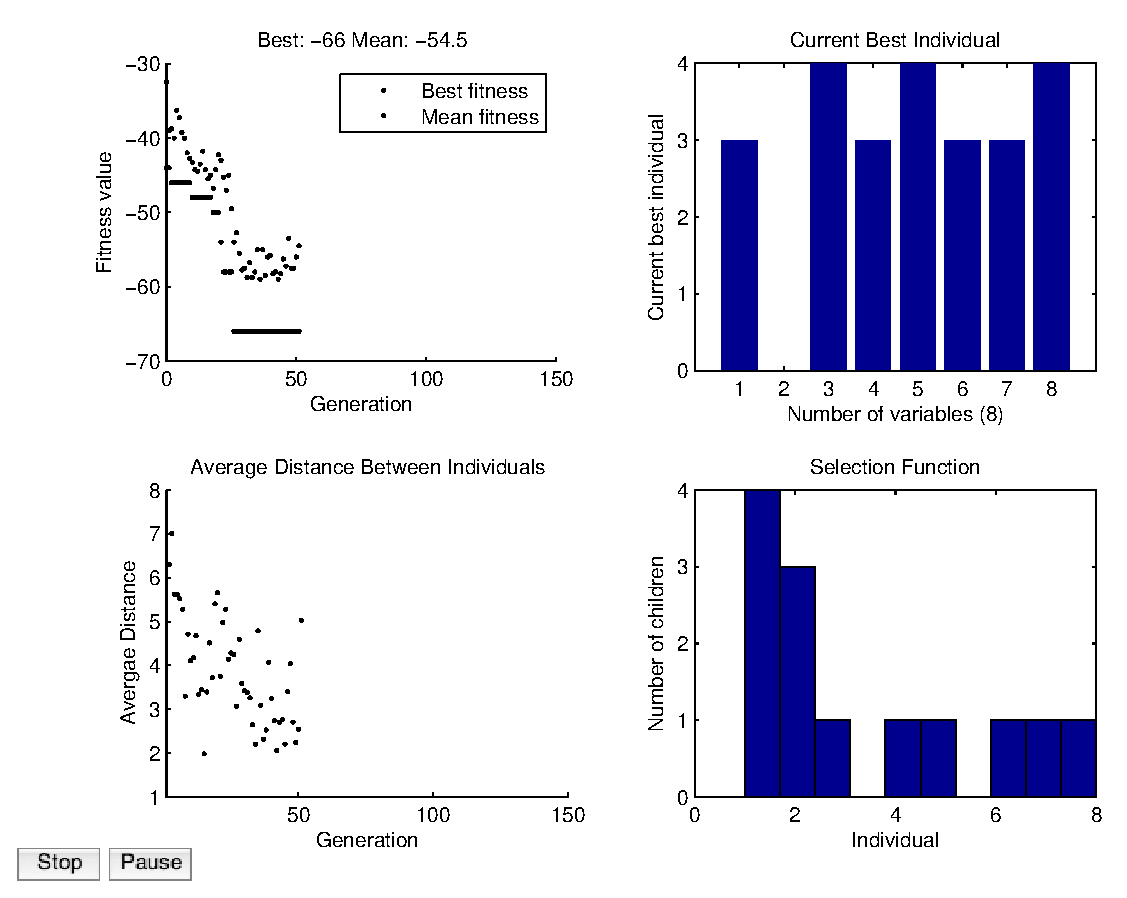
\includegraphics[scale=0.75]{images/avalanche_results8.eps} \\
	\label{bfjoint}
The results for the branch number, avalanche, and nonlinearity measurements for a $2$-bit S-box over all possible permutations in the design variables. 
\end{center}

\begin{center}
	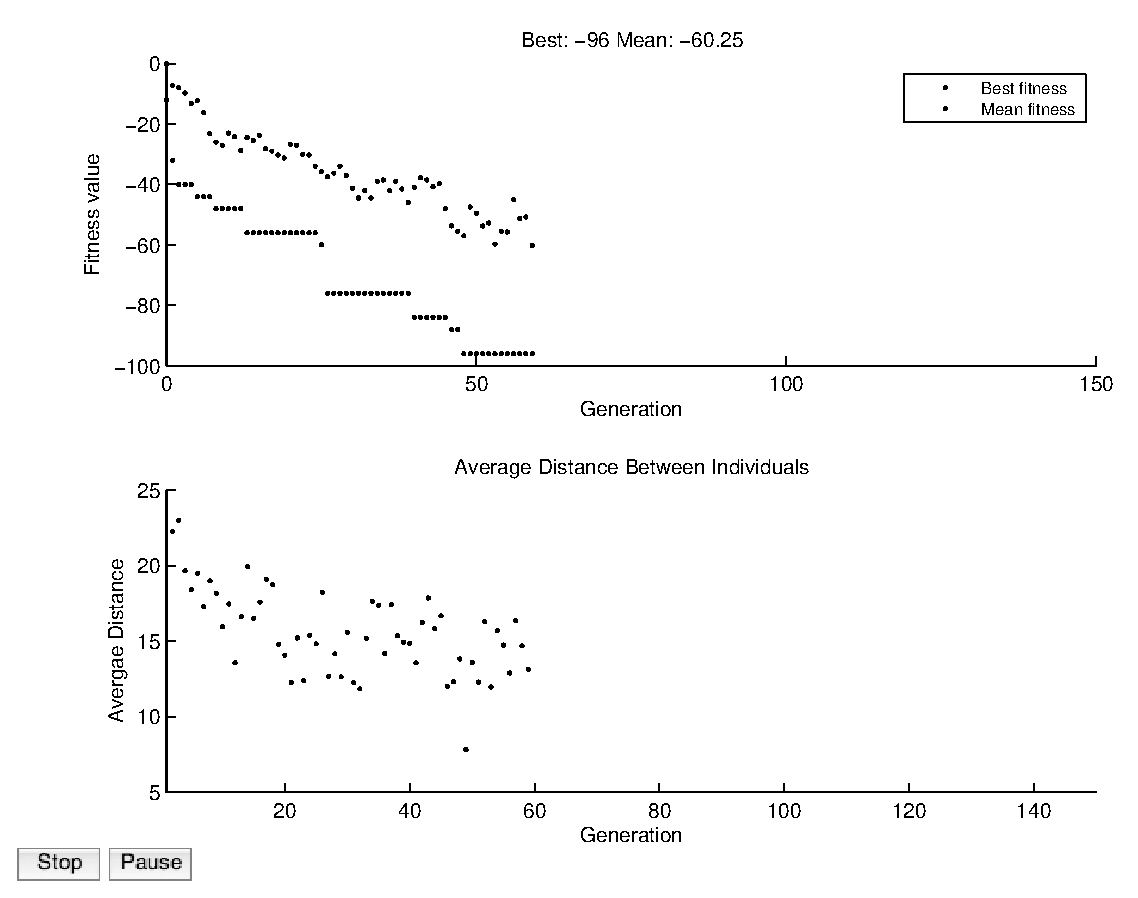
\includegraphics[scale=0.75]{images/avalanche_results16.eps} \\
	\label{bfjoint}
The results for the branch number, avalanche, and nonlinearity measurements for a $2$-bit S-box over all possible permutations in the design variables. 
\end{center}

\subsection{Branch Number}
TODO: insert code/charts

\begin{center}
	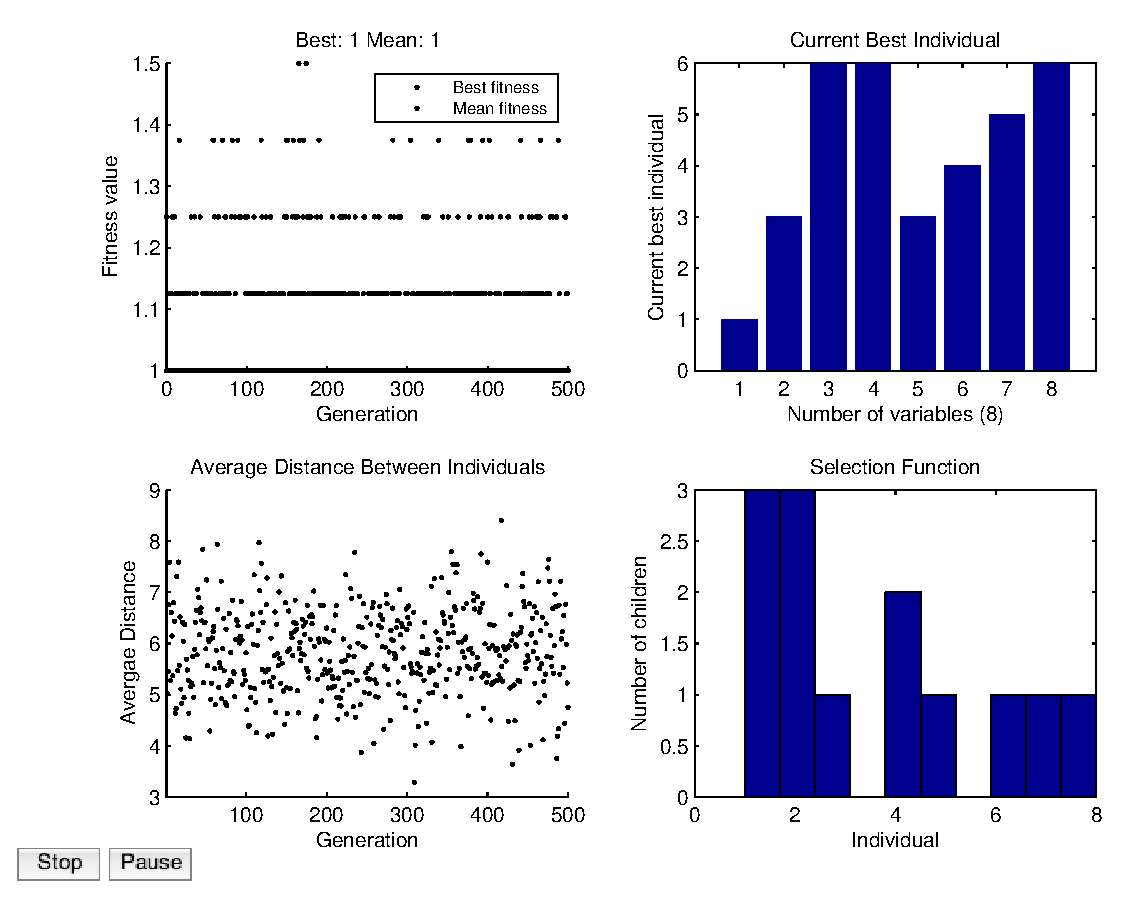
\includegraphics[scale=0.75]{images/bn_results8.eps} \\
	\label{bfjoint}
The results for the branch number, avalanche, and nonlinearity measurements for a $2$-bit S-box over all possible permutations in the design variables. 
\end{center}

\begin{center}
	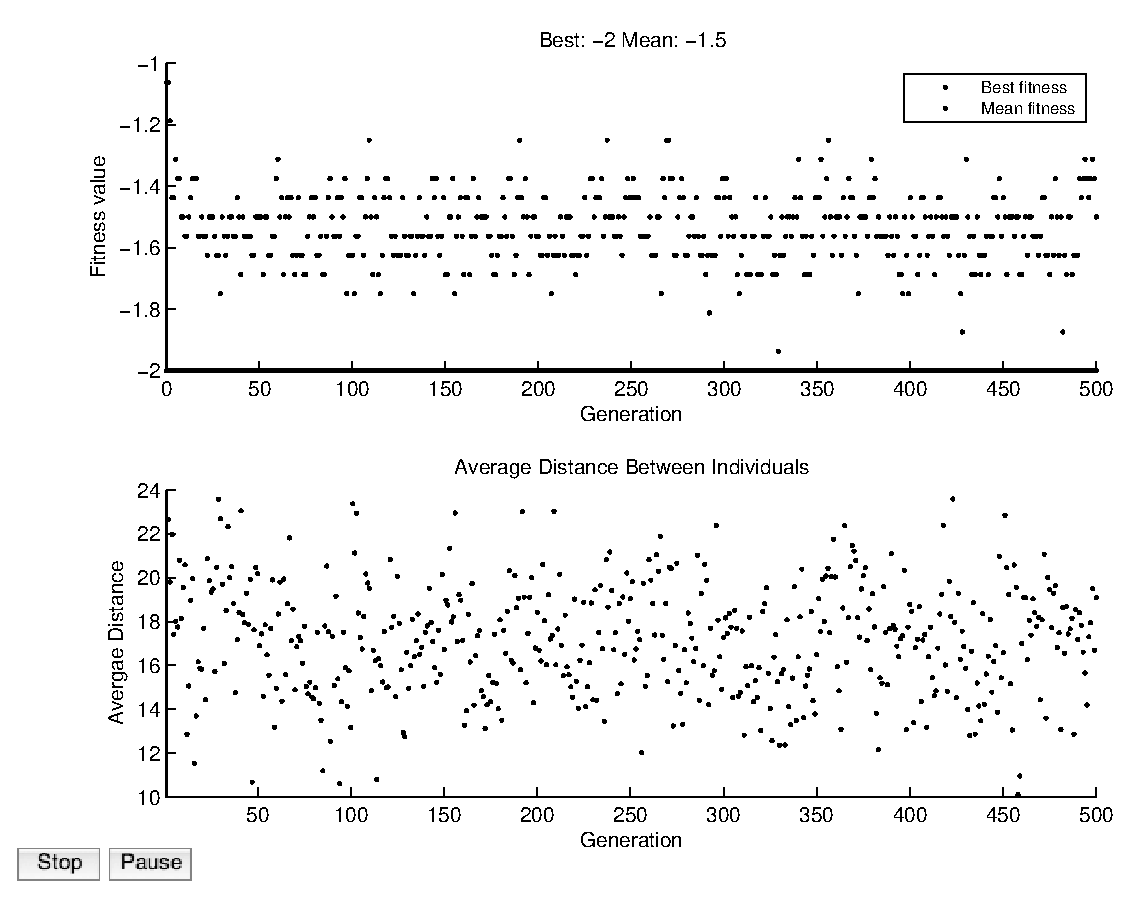
\includegraphics[scale=0.75]{images/bn_results16.eps} \\
	\label{bfjoint}
The results for the branch number, avalanche, and nonlinearity measurements for a $2$-bit S-box over all possible permutations in the design variables. 
\end{center}

\subsection{Nonlinearity Measurement}
TODO: insert code/charts

\begin{center}
	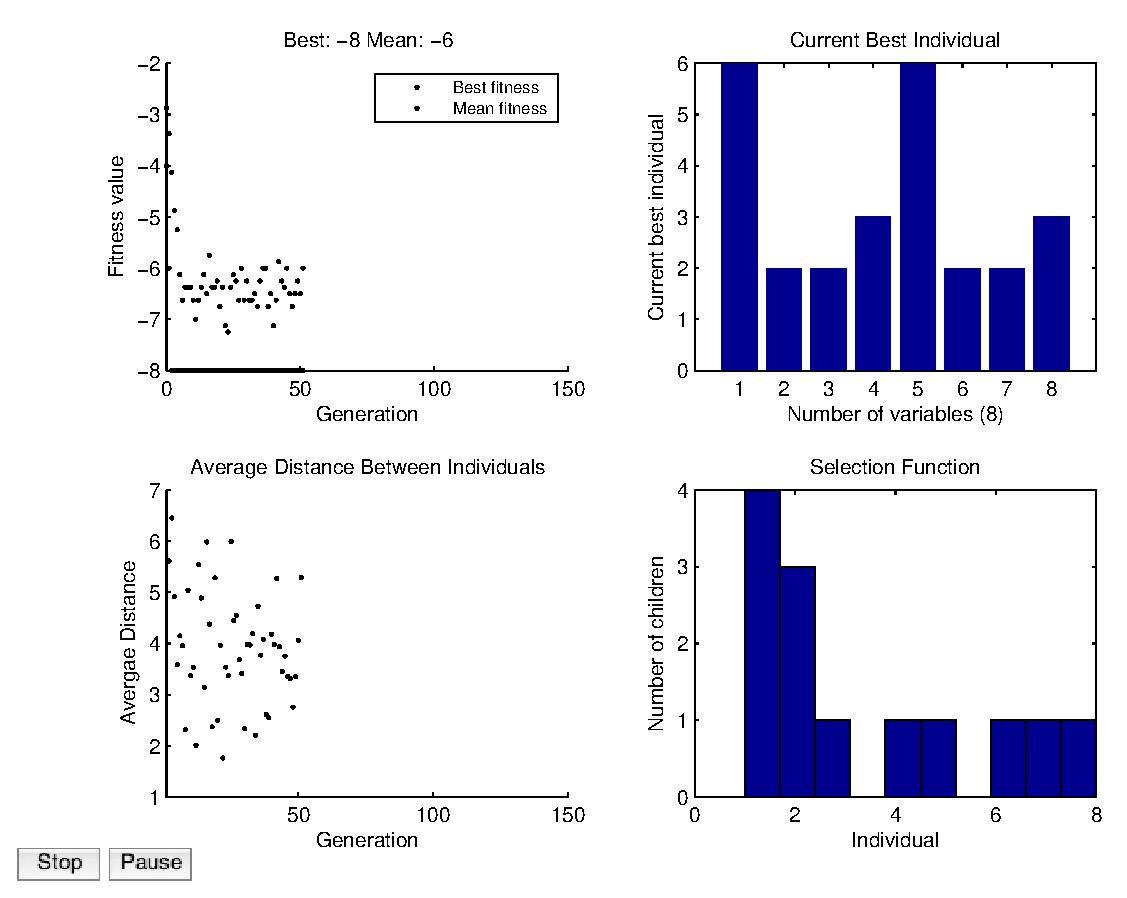
\includegraphics[scale=0.75]{images/nl_results8.eps} \\
	\label{bfjoint}
The results for the branch number, avalanche, and nonlinearity measurements for a $2$-bit S-box over all possible permutations in the design variables. 
\end{center}

\begin{center}
	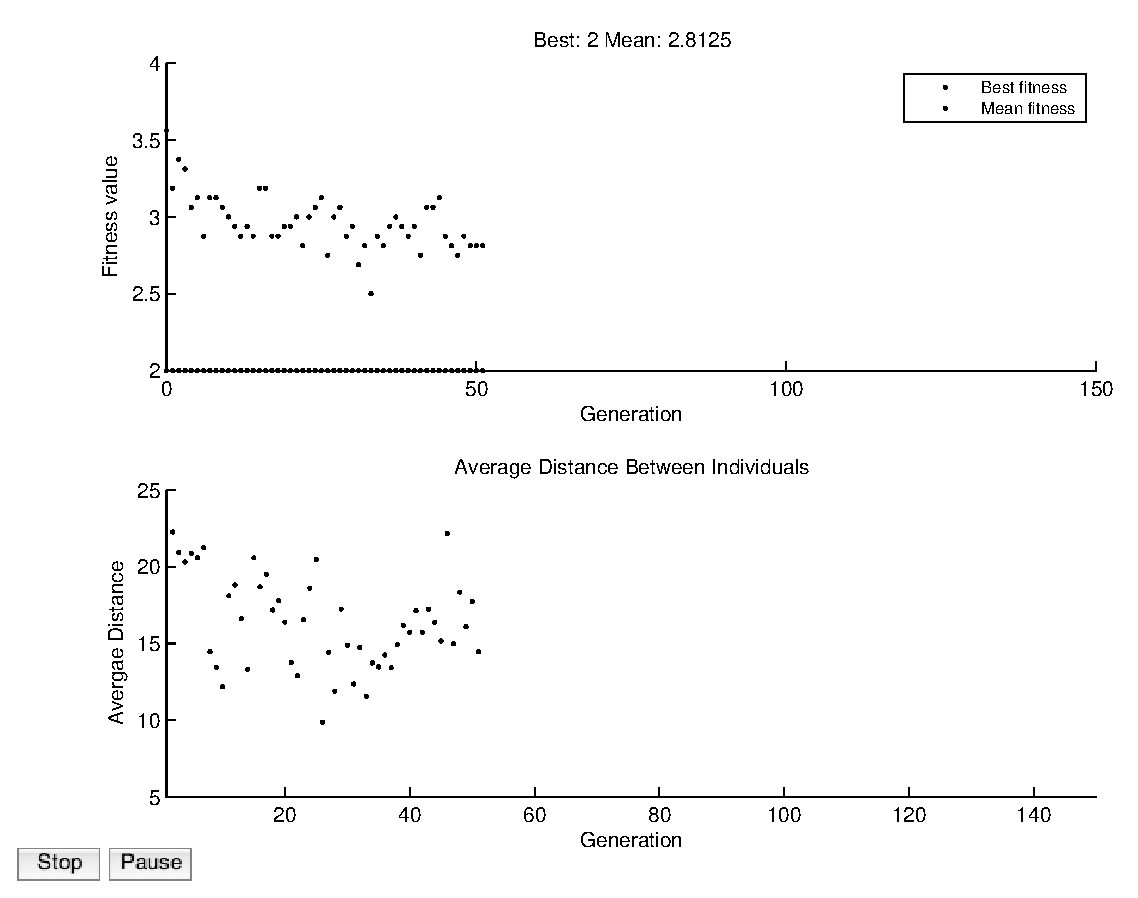
\includegraphics[scale=0.75]{images/nl_results16.eps} \\
	\label{bfjoint}
The results for the branch number, avalanche, and nonlinearity measurements for a $2$-bit S-box over all possible permutations in the design variables. 
\end{center}

\subsection{Multi-Objective Optimization}
Based on the fact that cryptographers and mathematicians attempt to optimize all of these measurements together, it is ideal to find an optimal value among all of the objective functions simultaneously. The most common way to solve this is to re-write the optimization problem as a linear combination of all three objective functions. The benefit of this approach is that we can prioritize the influence that each objective function has on the overall solution by assigning weights to each value in this linear combination. For the purposes of this project, the following linear combination was used to construct the multi-objective MINLP problem.

TODO: write the stuff here

% http://www.reveresecurity.com/_pdfs/s4x4Analysis.pdf
% says that BN must be at least 2 for bijective S-boxes

\section{Conclusions and Future Work}
%TODO: GA was most promising - similar to BF approach
%TODO: results were closest to brute force, and presumed to be close to actual values
%TODO: joint computations using GA were ineffective, exhaustive searches would be better, contradicting functions caused too great penalties and little change in design variabes
%TODO:  GA work - tweak crossover and mutation functions, run on large scale hardware/software systems

\bibliographystyle{IEEEtran}
% argument is your BibTeX string definitions and bibliography database(s)
\bibliography{caw4567-report-final}

\end{document}
